% Options for packages loaded elsewhere
\PassOptionsToPackage{unicode}{hyperref}
\PassOptionsToPackage{hyphens}{url}
\PassOptionsToPackage{dvipsnames,svgnames*,x11names*}{xcolor}
%
\documentclass[
]{article}
\usepackage{lmodern}
\usepackage{amssymb,amsmath}
\usepackage{ifxetex,ifluatex}
\ifnum 0\ifxetex 1\fi\ifluatex 1\fi=0 % if pdftex
  \usepackage[T1]{fontenc}
  \usepackage[utf8]{inputenc}
  \usepackage{textcomp} % provide euro and other symbols
\else % if luatex or xetex
  \usepackage{unicode-math}
  \defaultfontfeatures{Scale=MatchLowercase}
  \defaultfontfeatures[\rmfamily]{Ligatures=TeX,Scale=1}
\fi
% Use upquote if available, for straight quotes in verbatim environments
\IfFileExists{upquote.sty}{\usepackage{upquote}}{}
\IfFileExists{microtype.sty}{% use microtype if available
  \usepackage[]{microtype}
  \UseMicrotypeSet[protrusion]{basicmath} % disable protrusion for tt fonts
}{}
\makeatletter
\@ifundefined{KOMAClassName}{% if non-KOMA class
  \IfFileExists{parskip.sty}{%
    \usepackage{parskip}
  }{% else
    \setlength{\parindent}{0pt}
    \setlength{\parskip}{6pt plus 2pt minus 1pt}}
}{% if KOMA class
  \KOMAoptions{parskip=half}}
\makeatother
\usepackage{xcolor}
\IfFileExists{xurl.sty}{\usepackage{xurl}}{} % add URL line breaks if available
\IfFileExists{bookmark.sty}{\usepackage{bookmark}}{\usepackage{hyperref}}
\hypersetup{
  pdftitle={ESM 211 Homework 1},
  pdfauthor={Kelsie Fronheiser},
  colorlinks=true,
  linkcolor=Maroon,
  filecolor=Maroon,
  citecolor=Blue,
  urlcolor=blue,
  pdfcreator={LaTeX via pandoc}}
\urlstyle{same} % disable monospaced font for URLs
\usepackage[margin=1in]{geometry}
\usepackage{color}
\usepackage{fancyvrb}
\newcommand{\VerbBar}{|}
\newcommand{\VERB}{\Verb[commandchars=\\\{\}]}
\DefineVerbatimEnvironment{Highlighting}{Verbatim}{commandchars=\\\{\}}
% Add ',fontsize=\small' for more characters per line
\usepackage{framed}
\definecolor{shadecolor}{RGB}{248,248,248}
\newenvironment{Shaded}{\begin{snugshade}}{\end{snugshade}}
\newcommand{\AlertTok}[1]{\textcolor[rgb]{0.94,0.16,0.16}{#1}}
\newcommand{\AnnotationTok}[1]{\textcolor[rgb]{0.56,0.35,0.01}{\textbf{\textit{#1}}}}
\newcommand{\AttributeTok}[1]{\textcolor[rgb]{0.77,0.63,0.00}{#1}}
\newcommand{\BaseNTok}[1]{\textcolor[rgb]{0.00,0.00,0.81}{#1}}
\newcommand{\BuiltInTok}[1]{#1}
\newcommand{\CharTok}[1]{\textcolor[rgb]{0.31,0.60,0.02}{#1}}
\newcommand{\CommentTok}[1]{\textcolor[rgb]{0.56,0.35,0.01}{\textit{#1}}}
\newcommand{\CommentVarTok}[1]{\textcolor[rgb]{0.56,0.35,0.01}{\textbf{\textit{#1}}}}
\newcommand{\ConstantTok}[1]{\textcolor[rgb]{0.00,0.00,0.00}{#1}}
\newcommand{\ControlFlowTok}[1]{\textcolor[rgb]{0.13,0.29,0.53}{\textbf{#1}}}
\newcommand{\DataTypeTok}[1]{\textcolor[rgb]{0.13,0.29,0.53}{#1}}
\newcommand{\DecValTok}[1]{\textcolor[rgb]{0.00,0.00,0.81}{#1}}
\newcommand{\DocumentationTok}[1]{\textcolor[rgb]{0.56,0.35,0.01}{\textbf{\textit{#1}}}}
\newcommand{\ErrorTok}[1]{\textcolor[rgb]{0.64,0.00,0.00}{\textbf{#1}}}
\newcommand{\ExtensionTok}[1]{#1}
\newcommand{\FloatTok}[1]{\textcolor[rgb]{0.00,0.00,0.81}{#1}}
\newcommand{\FunctionTok}[1]{\textcolor[rgb]{0.00,0.00,0.00}{#1}}
\newcommand{\ImportTok}[1]{#1}
\newcommand{\InformationTok}[1]{\textcolor[rgb]{0.56,0.35,0.01}{\textbf{\textit{#1}}}}
\newcommand{\KeywordTok}[1]{\textcolor[rgb]{0.13,0.29,0.53}{\textbf{#1}}}
\newcommand{\NormalTok}[1]{#1}
\newcommand{\OperatorTok}[1]{\textcolor[rgb]{0.81,0.36,0.00}{\textbf{#1}}}
\newcommand{\OtherTok}[1]{\textcolor[rgb]{0.56,0.35,0.01}{#1}}
\newcommand{\PreprocessorTok}[1]{\textcolor[rgb]{0.56,0.35,0.01}{\textit{#1}}}
\newcommand{\RegionMarkerTok}[1]{#1}
\newcommand{\SpecialCharTok}[1]{\textcolor[rgb]{0.00,0.00,0.00}{#1}}
\newcommand{\SpecialStringTok}[1]{\textcolor[rgb]{0.31,0.60,0.02}{#1}}
\newcommand{\StringTok}[1]{\textcolor[rgb]{0.31,0.60,0.02}{#1}}
\newcommand{\VariableTok}[1]{\textcolor[rgb]{0.00,0.00,0.00}{#1}}
\newcommand{\VerbatimStringTok}[1]{\textcolor[rgb]{0.31,0.60,0.02}{#1}}
\newcommand{\WarningTok}[1]{\textcolor[rgb]{0.56,0.35,0.01}{\textbf{\textit{#1}}}}
\usepackage{graphicx,grffile}
\makeatletter
\def\maxwidth{\ifdim\Gin@nat@width>\linewidth\linewidth\else\Gin@nat@width\fi}
\def\maxheight{\ifdim\Gin@nat@height>\textheight\textheight\else\Gin@nat@height\fi}
\makeatother
% Scale images if necessary, so that they will not overflow the page
% margins by default, and it is still possible to overwrite the defaults
% using explicit options in \includegraphics[width, height, ...]{}
\setkeys{Gin}{width=\maxwidth,height=\maxheight,keepaspectratio}
% Set default figure placement to htbp
\makeatletter
\def\fps@figure{htbp}
\makeatother
\setlength{\emergencystretch}{3em} % prevent overfull lines
\providecommand{\tightlist}{%
  \setlength{\itemsep}{0pt}\setlength{\parskip}{0pt}}
\setcounter{secnumdepth}{-\maxdimen} % remove section numbering

\title{ESM 211 Homework 1}
\author{Kelsie Fronheiser}
\date{Due 15 Jan.~2021, 5 PM}

\begin{document}
\maketitle

\emph{Please upload your solutions to GauchoSpace as a pdf file. If you
used R or Rmarkdown, show the code chunks, except in the final ``report
to the park superintendant''.}

\emph{The data files are together with this file in the assigment
activity. I've also uploaded the .Rmd file that generated this file, if
you'd like to use it as a starting point for your solutions.}

Plants and animals are often distributed unevenly across space, even at
a local scale. This figure, which maps a hypothetical population, shows
a type of pattern that we often see:

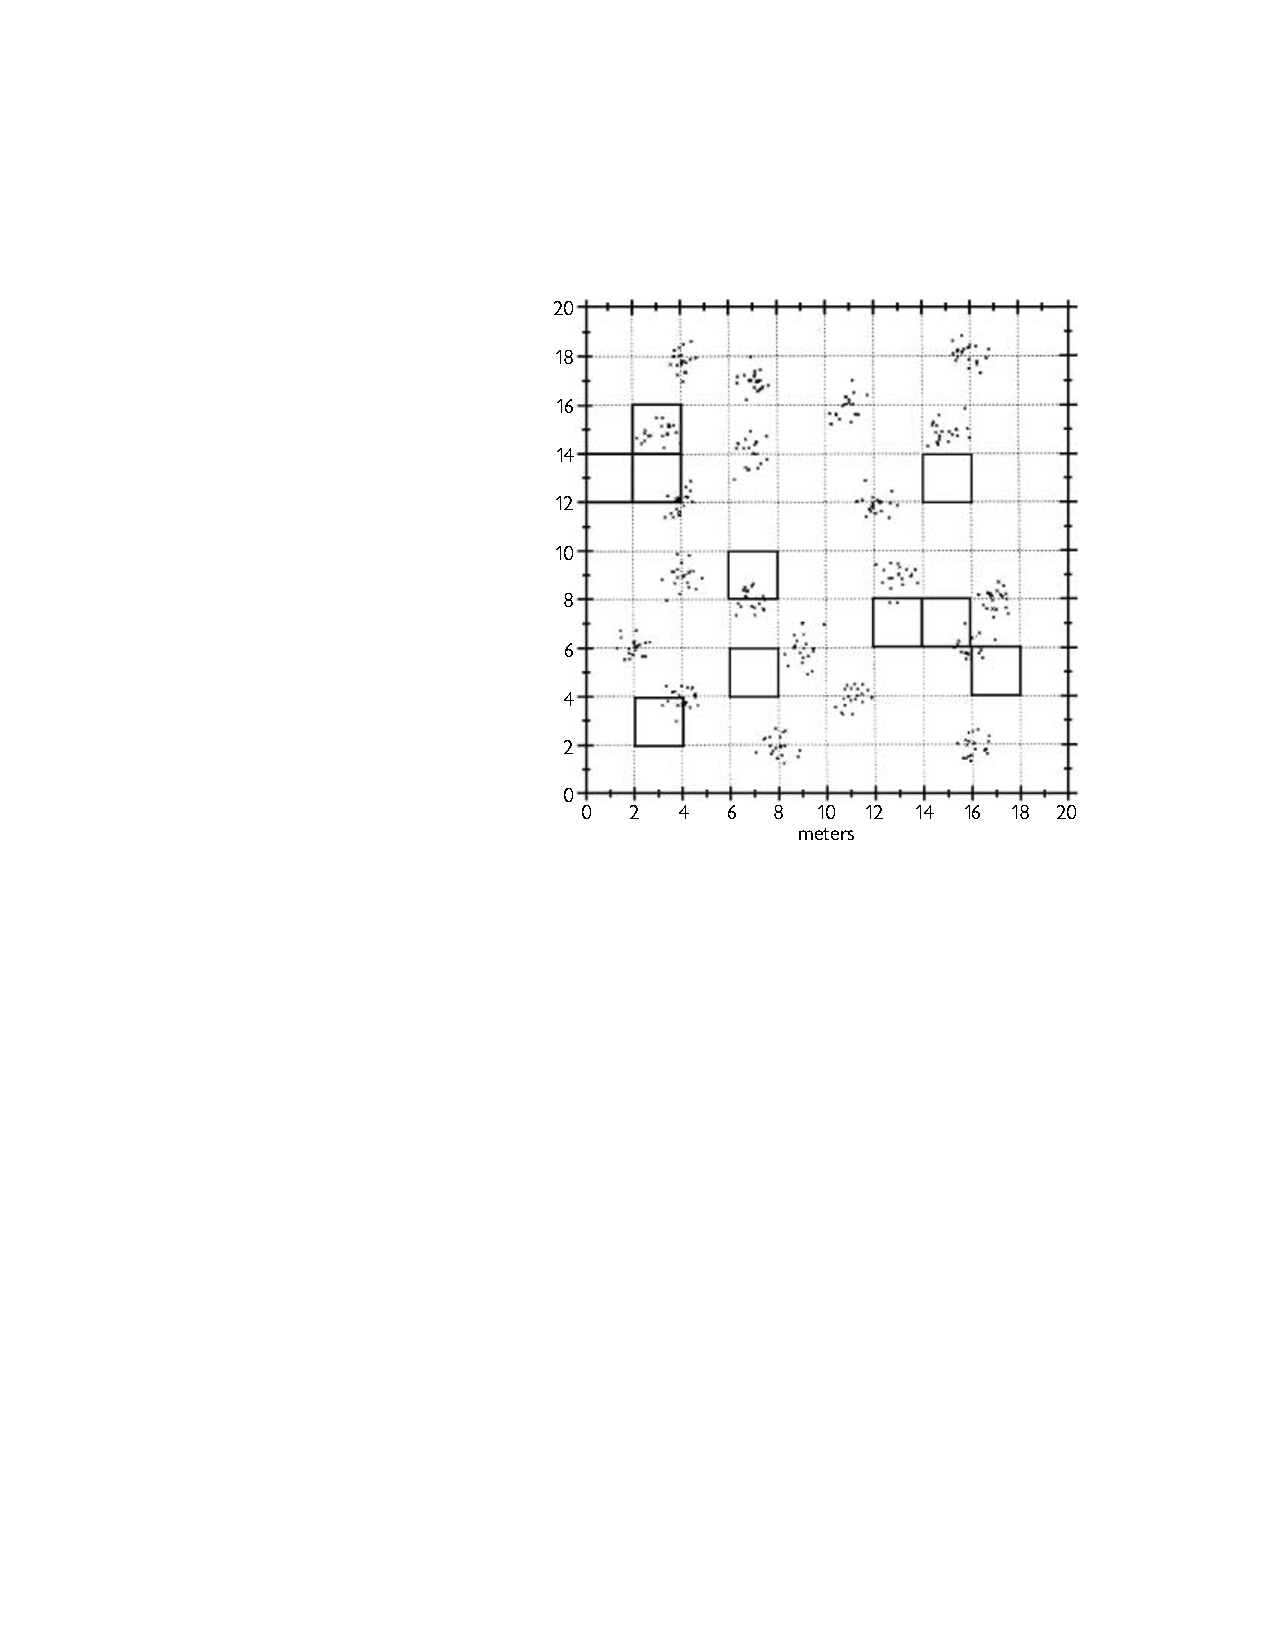
\includegraphics{../../Figures/Elzinga_1998_plant_map.pdf}

\emph{1. Give three reasons why a plant or animal might be patchily
distributed like this. For each, describe whether you would expect the
location of the high-density patches to be consistent from year to year
(3 points).}

\begin{enumerate}
\def\labelenumi{\arabic{enumi}.}
\item
  Particular biotic conditions (vegetation, animal species, fungi, etc)
  may be needed for a particular species, which would distribute the
  individuals to those particular areas. For example, certain bird
  species may only forage or nest in one or two tree species so they
  would be located in those individual trees and nowhere else in a
  landscape. In this case the location of the high-density patches would
  likely stay consistent from year to year unless there is a disturbance
  that disrupts the biotic condition(s) (i.e wildfire).
\item
  Particular abiotic conditions (temperature, slope, substrate,
  nutrients, etc) may be needed for a particular species, which would
  distribute the individuals to those particular areas. For example,a
  plant that needs a minimum amount of a certain nutrient, like
  phosphorus, to grow will only grow in areas where the substrate holds
  at least the minimum amount of phosphorous needed for that plant. In
  this case the high-density patches are likely to stay consistent from
  year to year.
\item
  Certain species may grow in aggregations and/or live in smaller
  subdivided social groups. Certain species are adapted to grow or live
  in groups for reasons such as protection, social behaviors,
  reproduction, etc. In this case the high-density patches are likely to
  change locations from year to year (although over a much longer time
  scale for plants rather than animals).
\end{enumerate}

\hypertarget{eureka-dune-grass}{%
\section{Eureka dune grass}\label{eureka-dune-grass}}

\href{https://calscape.org/Swallenia-alexandrae-()}{Eureka dune grass}
(\emph{Swallenia alexandrae}) is a rare bunchgrass that only grows on
\href{https://www.nps.gov/deva/planyourvisit/eureka-dunes.htm}{three
sand dunes} in Death Valley National Park. You are going to evaluate the
population change on one of those dunes (Saline Dune) from 2008 to 2011.

Plants were counted in 11 quadrats (each 1 ha) across the dune. The same
plots were used each year. The data are in the file
\texttt{Swallenia\_wide.csv} and \texttt{Swallenia\_long.csv} (the data
are the same; I've just provided wide and long formats so that you don't
need to deal with pivoting).

\begin{enumerate}
\def\labelenumi{\arabic{enumi}.}
\setcounter{enumi}{1}
\tightlist
\item
  Read in the data, and calculate the mean and standard error of
  \emph{Swallenia} density (plants/ha) in each year. Make a plot showing
  the means as points and the standard errors as error bars. Based on
  this plot, do you think that the \emph{Swallenia} population density
  has changed over time? (2 points)
\end{enumerate}

\begin{Shaded}
\begin{Highlighting}[]
\NormalTok{dunegrass <-}\StringTok{ }\KeywordTok{read.csv}\NormalTok{(}\StringTok{"Swallenia_long.csv"}\NormalTok{)}

\NormalTok{dunegrass_mean <-}\StringTok{ }\NormalTok{dunegrass }\OperatorTok
\StringTok{  }\KeywordTok{group_by}\NormalTok{(year) }\OperatorTok
\StringTok{  }\KeywordTok{summarise}\NormalTok{(}\DataTypeTok{sum =} \KeywordTok{sum}\NormalTok{(count),}
            \DataTypeTok{mean =} \KeywordTok{mean}\NormalTok{(count),}
            \DataTypeTok{sd =} \KeywordTok{sd}\NormalTok{(count, }\DataTypeTok{na.rm =} \OtherTok{TRUE}\NormalTok{),}
              \DataTypeTok{se =} \KeywordTok{sd}\NormalTok{(count) }\OperatorTok{/}\StringTok{ }\KeywordTok{sqrt}\NormalTok{(}\KeywordTok{n}\NormalTok{()))}
\end{Highlighting}
\end{Shaded}

\begin{verbatim}
## `summarise()` ungrouping output (override with `.groups` argument)
\end{verbatim}

\begin{Shaded}
\begin{Highlighting}[]
\KeywordTok{ggplot}\NormalTok{(}\DataTypeTok{data =}\NormalTok{ dunegrass_mean, }\KeywordTok{aes}\NormalTok{(}\DataTypeTok{x =}\NormalTok{ year, }\DataTypeTok{y =}\NormalTok{ mean)) }\OperatorTok{+}
\StringTok{         }\KeywordTok{geom_point}\NormalTok{(}\DataTypeTok{size =} \DecValTok{3}\NormalTok{) }\OperatorTok{+}\StringTok{ }
\StringTok{ }\KeywordTok{geom_errorbar}\NormalTok{(}\KeywordTok{aes}\NormalTok{(}\DataTypeTok{x =}\NormalTok{ year, }\DataTypeTok{ymin =}\NormalTok{ mean }\OperatorTok{-}\StringTok{ }\NormalTok{se, }\DataTypeTok{ymax =}\NormalTok{ mean }\OperatorTok{+}\StringTok{ }\NormalTok{se), }\DataTypeTok{width =} \FloatTok{0.1}\NormalTok{, }\DataTypeTok{color =} \StringTok{"darkred"}\NormalTok{, }\DataTypeTok{size =} \FloatTok{1.3}\NormalTok{) }\OperatorTok{+}
\StringTok{ }\KeywordTok{labs}\NormalTok{(}\DataTypeTok{title =} \StringTok{"*Swallenia* Desnsity Over Time"}\NormalTok{, }\DataTypeTok{x =} \StringTok{"Year"}\NormalTok{, }\DataTypeTok{y =} \StringTok{"Mean *Swallenia* Density (plants/ha)"}\NormalTok{, }\DataTypeTok{caption =} \StringTok{"Mean density for *Swallenia* Dengrass is shown as black points for each year, with the standard error of the mean shown }\CharTok{\textbackslash{}n}\StringTok{ as red errorbars."}\NormalTok{) }\OperatorTok{+}
\StringTok{  }\KeywordTok{theme_minimal}\NormalTok{()}
\end{Highlighting}
\end{Shaded}

\includegraphics{HW1_files/figure-latex/unnamed-chunk-1-1.pdf} I do
think that the \emph{Swallenia} population density has changed over
time.

\hypertarget{arithmetic-growth-rate}{%
\subsection{Arithmetic growth rate}\label{arithmetic-growth-rate}}

With four years of data, we can calculate three annual population growth
rates (2008-09, 2009-10, and 2010-11). We'll start with the arithmetic
growth rate, which you should recall is the difference in abundance
divided by the time interval.

\begin{enumerate}
\def\labelenumi{\arabic{enumi}.}
\setcounter{enumi}{2}
\tightlist
\item
  Using the mean densities from the prior question, what are the
  estimated growth rates for each of the three annual timesteps? (1
  point)
\end{enumerate}

\begin{Shaded}
\begin{Highlighting}[]
\NormalTok{EGR2008_}\DecValTok{2009}\NormalTok{ <-}\StringTok{ }\NormalTok{(}\FloatTok{61.90909} \OperatorTok{-}\StringTok{ }\FloatTok{56.27273}\NormalTok{) }\OperatorTok{/}\DecValTok{1}
\NormalTok{EGR2009_}\DecValTok{2010}\NormalTok{ <-}\StringTok{ }\NormalTok{(}\FloatTok{101.36364} \OperatorTok{-}\StringTok{ }\FloatTok{61.90909}\NormalTok{) }\OperatorTok{/}\DecValTok{1}
\NormalTok{EGR2010_}\DecValTok{2011}\NormalTok{ <-}\StringTok{ }\NormalTok{(}\FloatTok{69.45455} \OperatorTok{-}\StringTok{ }\FloatTok{101.36364}\NormalTok{) }\OperatorTok{/}\DecValTok{1}
  
\NormalTok{EGR2008_}\DecValTok{2009}
\end{Highlighting}
\end{Shaded}

\begin{verbatim}
## [1] 5.63636
\end{verbatim}

\begin{Shaded}
\begin{Highlighting}[]
\NormalTok{EGR2009_}\DecValTok{2010}
\end{Highlighting}
\end{Shaded}

\begin{verbatim}
## [1] 39.45455
\end{verbatim}

\begin{Shaded}
\begin{Highlighting}[]
\NormalTok{EGR2010_}\DecValTok{2011}
\end{Highlighting}
\end{Shaded}

\begin{verbatim}
## [1] -31.90909
\end{verbatim}

\begin{Shaded}
\begin{Highlighting}[]
\NormalTok{EGR <-}\StringTok{ }\NormalTok{dunegrass_mean }\OperatorTok\StringTok{ }
\StringTok{  }\KeywordTok{mutate}\NormalTok{(}\DataTypeTok{Estimated_GR =} \KeywordTok{lead}\NormalTok{(mean) }\OperatorTok{-}\StringTok{ }\NormalTok{mean }\OperatorTok{/}\DecValTok{1}\NormalTok{ )}
\end{Highlighting}
\end{Shaded}

\begin{enumerate}
\def\labelenumi{\arabic{enumi}.}
\setcounter{enumi}{3}
\tightlist
\item
  Given the within-year variability in the abundance estimates, we might
  wonder whether there is statistical evidence that the growth rates are
  different from zero. A t-test can give us an answer to this. However,
  you need to decide whether a two-sample t-test or a paired t-test is
  more appropriate to use. Thinking about the structure of the data, as
  well as your answers to the first question, choose one of these tests
  and explain why it is most appropriate. Even if neither is perfect,
  you still need to choose the ``least bad'' one. (2 points)
\end{enumerate}

I think a paired t-test is the best option.

\begin{enumerate}
\def\labelenumi{\arabic{enumi}.}
\setcounter{enumi}{4}
\tightlist
\item
  Based on your decision in the previous question, use either two-sample
  t-tests or paired t-tests to evaluate whether there is evidence that
  the population growth rate was different from zero in each of the
  three years (you'll need to run separate tests for each of 2008-09,
  2009-10, and 2010-11). Choose a level for \(\alpha\), and justify your
  choice. Based on the P-values, in which (if any) years can you reject
  the null hypothesis that the growth rate is zero? (2 points)
\end{enumerate}

Recall that you can do a t-test in R using \texttt{t.test()}, and that
you use \texttt{paired\ =\ TRUE} to do a paired test. You can set
\(\alpha\) using the \texttt{conf.level} argument. Also, be aware that
\texttt{t.test(x,\ y)} gives you the mean value of \(x - y\), so choose
your data subsets accordingly.

\begin{Shaded}
\begin{Highlighting}[]
\NormalTok{dunegrass1 <-}\StringTok{ }\KeywordTok{read_csv}\NormalTok{(}\StringTok{"Swallenia_wide.csv"}\NormalTok{)}
\end{Highlighting}
\end{Shaded}

\begin{verbatim}
## 
## -- Column specification --------------------------------------------------------
## cols(
##   plot = col_character(),
##   count_2008 = col_double(),
##   count_2009 = col_double(),
##   count_2010 = col_double(),
##   count_2011 = col_double()
## )
\end{verbatim}

\begin{Shaded}
\begin{Highlighting}[]
\NormalTok{count2008 <-}\StringTok{ }\NormalTok{dunegrass }\OperatorTok\StringTok{ }
\StringTok{  }\KeywordTok{filter}\NormalTok{(year }\OperatorTok{==}\StringTok{ "2008"}\NormalTok{)}

\NormalTok{count2009 <-}\StringTok{ }\NormalTok{dunegrass }\OperatorTok\StringTok{ }
\StringTok{  }\KeywordTok{filter}\NormalTok{(year }\OperatorTok{==}\StringTok{ "2009"}\NormalTok{)}

\NormalTok{ttest2008_}\DecValTok{2009}\NormalTok{ <-}\StringTok{ }\KeywordTok{t.test}\NormalTok{(}\DataTypeTok{x =}\NormalTok{ count2009}\OperatorTok{$}\NormalTok{count,}\DataTypeTok{y =}\NormalTok{ count2008}\OperatorTok{$}\NormalTok{count, }\DataTypeTok{paired =} \OtherTok{TRUE}\NormalTok{, }\DataTypeTok{conf.level =} \FloatTok{0.95}\NormalTok{) }

\NormalTok{count2010 <-}\StringTok{ }\NormalTok{dunegrass }\OperatorTok\StringTok{ }
\StringTok{  }\KeywordTok{filter}\NormalTok{(year }\OperatorTok{==}\StringTok{ "2010"}\NormalTok{)}

\NormalTok{count2011 <-}\StringTok{ }\NormalTok{dunegrass }\OperatorTok\StringTok{ }
\StringTok{  }\KeywordTok{filter}\NormalTok{(year }\OperatorTok{==}\StringTok{ "2011"}\NormalTok{)}

\NormalTok{ttest2009_}\DecValTok{2010}\NormalTok{ <-}\StringTok{ }\KeywordTok{t.test}\NormalTok{(}\DataTypeTok{x =}\NormalTok{ count2010}\OperatorTok{$}\NormalTok{count,}\DataTypeTok{y =}\NormalTok{ count2009}\OperatorTok{$}\NormalTok{count, }\DataTypeTok{paired =} \OtherTok{TRUE}\NormalTok{, }\DataTypeTok{conf.level =} \FloatTok{0.95}\NormalTok{) }

\NormalTok{ttest2010_}\DecValTok{2011}\NormalTok{ <-}\StringTok{ }\KeywordTok{t.test}\NormalTok{(}\DataTypeTok{x =}\NormalTok{ count2011}\OperatorTok{$}\NormalTok{count,}\DataTypeTok{y =}\NormalTok{ count2010}\OperatorTok{$}\NormalTok{count, }\DataTypeTok{paired =} \OtherTok{TRUE}\NormalTok{, }\DataTypeTok{conf.level =} \FloatTok{0.95}\NormalTok{) }

\NormalTok{ttest2008_}\DecValTok{2009}
\end{Highlighting}
\end{Shaded}

\begin{verbatim}
## 
##  Paired t-test
## 
## data:  count2009$count and count2008$count
## t = 0.98217, df = 10, p-value = 0.3492
## alternative hypothesis: true difference in means is not equal to 0
## 95 percent confidence interval:
##  -7.15017 18.42290
## sample estimates:
## mean of the differences 
##                5.636364
\end{verbatim}

\begin{Shaded}
\begin{Highlighting}[]
\NormalTok{ttest2009_}\DecValTok{2010}
\end{Highlighting}
\end{Shaded}

\begin{verbatim}
## 
##  Paired t-test
## 
## data:  count2010$count and count2009$count
## t = 2.4508, df = 10, p-value = 0.03421
## alternative hypothesis: true difference in means is not equal to 0
## 95 percent confidence interval:
##   3.584261 75.324830
## sample estimates:
## mean of the differences 
##                39.45455
\end{verbatim}

\begin{Shaded}
\begin{Highlighting}[]
\NormalTok{ttest2010_}\DecValTok{2011}
\end{Highlighting}
\end{Shaded}

\begin{verbatim}
## 
##  Paired t-test
## 
## data:  count2011$count and count2010$count
## t = -2.4037, df = 10, p-value = 0.03708
## alternative hypothesis: true difference in means is not equal to 0
## 95 percent confidence interval:
##  -61.487703  -2.330479
## sample estimates:
## mean of the differences 
##               -31.90909
\end{verbatim}

\begin{enumerate}
\def\labelenumi{\arabic{enumi}.}
\setcounter{enumi}{5}
\tightlist
\item
  What assumptions does the t-test make about the normality of the data
  (note that this differs for the 2-sample and paired tests)? Do your
  data satisfy those assumptions? If not, how might that affect the
  interpretation of your results? (2 points)
\end{enumerate}

\hypertarget{log-growth-rate}{%
\subsection{Log growth rate}\label{log-growth-rate}}

The geometric growth rate, \(\lambda_t = \frac{N_{t+1}}{N_t}\), is
difficult to put uncertainty bounds on (the uncertainty in the
denominator has a strongly nonlinear effect on the overall ratio).
Instead, we look at the log growth rate,
\(r_t = \log \lambda_t = \log N_{t_1} - \log N_t\).

\begin{enumerate}
\def\labelenumi{\arabic{enumi}.}
\setcounter{enumi}{6}
\tightlist
\item
  For each of the three years, use the t-test (the same type that you
  previously chose), applied to the log transformation of the abundance
  data, to calculate the mean value of \(r_t\) and test the null
  hypothesis that it is zero. Based on the P-values, in which (if any)
  years can you reject the null hypothesis that the growth rate is zero?
  (2 points)
\end{enumerate}

\begin{Shaded}
\begin{Highlighting}[]
\NormalTok{log_transform <-dunegrass1 }\OperatorTok\StringTok{ }
\StringTok{  }\KeywordTok{mutate}\NormalTok{(}\DataTypeTok{log_08 =} \KeywordTok{log}\NormalTok{(count_}\DecValTok{2008}\NormalTok{),}
         \DataTypeTok{log_09 =} \KeywordTok{log}\NormalTok{(count_}\DecValTok{2009}\NormalTok{),}
         \DataTypeTok{log_10 =} \KeywordTok{log}\NormalTok{(count_}\DecValTok{2010}\NormalTok{),}
         \DataTypeTok{log_11 =} \KeywordTok{log}\NormalTok{(count_}\DecValTok{2011}\NormalTok{)) }\OperatorTok\StringTok{ }
\KeywordTok{select}\NormalTok{(plot, log_}\DecValTok{08}\OperatorTok{:}\NormalTok{log_}\DecValTok{11}\NormalTok{)}

\NormalTok{GGR <-}\StringTok{ }\NormalTok{dunegrass_mean }\OperatorTok\StringTok{ }
\StringTok{  }\KeywordTok{mutate}\NormalTok{(}\DataTypeTok{lamda_t =} \KeywordTok{lead}\NormalTok{(sum)}\OperatorTok{/}\NormalTok{sum) }\OperatorTok\StringTok{ }
\StringTok{  }\KeywordTok{mutate}\NormalTok{(}\DataTypeTok{R_T =} \KeywordTok{log}\NormalTok{(lamda_t))}

\KeywordTok{ggplot}\NormalTok{(}\DataTypeTok{data =}\NormalTok{ GGR, }\KeywordTok{aes}\NormalTok{(}\DataTypeTok{x =}\NormalTok{ year, }\DataTypeTok{y =}\NormalTok{ R_T)) }\OperatorTok{+}
\StringTok{  }\KeywordTok{geom_point}\NormalTok{()}
\end{Highlighting}
\end{Shaded}

\begin{verbatim}
## Warning: Removed 1 rows containing missing values (geom_point).
\end{verbatim}

\includegraphics{HW1_files/figure-latex/unnamed-chunk-4-1.pdf}

\begin{Shaded}
\begin{Highlighting}[]
\NormalTok{log2008 <-}\StringTok{ }\NormalTok{log_transform }\OperatorTok\StringTok{ }
\StringTok{  }\KeywordTok{select}\NormalTok{(}\StringTok{"log_08"}\NormalTok{)}

\NormalTok{log2009 <-}\StringTok{ }\NormalTok{log_transform }\OperatorTok\StringTok{ }
\StringTok{  }\KeywordTok{select}\NormalTok{(}\StringTok{"log_09"}\NormalTok{)}

\NormalTok{ttestlog2008_}\DecValTok{2009}\NormalTok{ <-}\StringTok{ }\KeywordTok{t.test}\NormalTok{(}\DataTypeTok{x =}\NormalTok{ log2009}\OperatorTok{$}\NormalTok{log_}\DecValTok{09}\NormalTok{,}\DataTypeTok{y =}\NormalTok{ log2008}\OperatorTok{$}\NormalTok{log_}\DecValTok{08}\NormalTok{, }\DataTypeTok{paired =} \OtherTok{TRUE}\NormalTok{, }\DataTypeTok{conf.level =} \FloatTok{0.95}\NormalTok{) }

\NormalTok{log2010 <-}\StringTok{ }\NormalTok{log_transform }\OperatorTok\StringTok{ }
\StringTok{  }\KeywordTok{select}\NormalTok{(}\StringTok{"log_10"}\NormalTok{)}

\NormalTok{log2011 <-}\StringTok{ }\NormalTok{log_transform }\OperatorTok\StringTok{ }
\StringTok{  }\KeywordTok{select}\NormalTok{(}\StringTok{"log_11"}\NormalTok{)}

\NormalTok{ttestlog2009_}\DecValTok{2010}\NormalTok{ <-}\StringTok{ }\KeywordTok{t.test}\NormalTok{(}\DataTypeTok{x =}\NormalTok{ log2010}\OperatorTok{$}\NormalTok{log_}\DecValTok{10}\NormalTok{,}\DataTypeTok{y =}\NormalTok{ log2009}\OperatorTok{$}\NormalTok{log_}\DecValTok{09}\NormalTok{, }\DataTypeTok{paired =} \OtherTok{TRUE}\NormalTok{, }\DataTypeTok{conf.level =} \FloatTok{0.95}\NormalTok{) }

\NormalTok{ttestlog2010_}\DecValTok{2011}\NormalTok{ <-}\StringTok{ }\KeywordTok{t.test}\NormalTok{(}\DataTypeTok{x =}\NormalTok{ log2011}\OperatorTok{$}\NormalTok{log_}\DecValTok{11}\NormalTok{,}\DataTypeTok{y =}\NormalTok{ log2010}\OperatorTok{$}\NormalTok{log_}\DecValTok{10}\NormalTok{, }\DataTypeTok{paired =} \OtherTok{TRUE}\NormalTok{, }\DataTypeTok{conf.level =} \FloatTok{0.95}\NormalTok{) }

\NormalTok{ttestlog2008_}\DecValTok{2009}
\end{Highlighting}
\end{Shaded}

\begin{verbatim}
## 
##  Paired t-test
## 
## data:  log2009$log_09 and log2008$log_08
## t = 1.3923, df = 10, p-value = 0.194
## alternative hypothesis: true difference in means is not equal to 0
## 95 percent confidence interval:
##  -0.1311869  0.5681997
## sample estimates:
## mean of the differences 
##               0.2185064
\end{verbatim}

\begin{Shaded}
\begin{Highlighting}[]
\NormalTok{ttestlog2009_}\DecValTok{2010}
\end{Highlighting}
\end{Shaded}

\begin{verbatim}
## 
##  Paired t-test
## 
## data:  log2010$log_10 and log2009$log_09
## t = 3.6538, df = 10, p-value = 0.004434
## alternative hypothesis: true difference in means is not equal to 0
## 95 percent confidence interval:
##  0.1515138 0.6251153
## sample estimates:
## mean of the differences 
##               0.3883146
\end{verbatim}

\begin{Shaded}
\begin{Highlighting}[]
\NormalTok{ttestlog2010_}\DecValTok{2011}
\end{Highlighting}
\end{Shaded}

\begin{verbatim}
## 
##  Paired t-test
## 
## data:  log2011$log_11 and log2010$log_10
## t = -4.0395, df = 10, p-value = 0.002363
## alternative hypothesis: true difference in means is not equal to 0
## 95 percent confidence interval:
##  -0.8041814 -0.2324079
## sample estimates:
## mean of the differences 
##              -0.5182946
\end{verbatim}

\begin{enumerate}
\def\labelenumi{\arabic{enumi}.}
\setcounter{enumi}{7}
\tightlist
\item
  Do the log-transformed data fit the normality assumptions of the
  t-test better or worse than the untransformed data? On the basis of
  this comparison, are you more confident about the statistical results
  for the arithmetic growth rate or the log growth rate? (2 points)
\end{enumerate}

\begin{Shaded}
\begin{Highlighting}[]
\NormalTok{log_transform1 <-}\StringTok{ }\KeywordTok{pivot_longer}\NormalTok{(log_transform, }
                               \DataTypeTok{cols =} \KeywordTok{starts_with}\NormalTok{(}\StringTok{"log"}\NormalTok{),}
                               \DataTypeTok{names_to =} \StringTok{"year"}\NormalTok{)}

\CommentTok{#ggplot(data = log_transform1, aes(x = year, y = value)) +}
  \CommentTok{#geom_qq(data = log_transform1, aes(x = year, sample = value, color = plot))}
\CommentTok{# geom_qq_line(data = log_transform1, aes(sample = value)) +}
  \CommentTok{#facet_wrap( ~ year)}

\NormalTok{qqlog <-}\StringTok{ }\KeywordTok{qqnorm}\NormalTok{(log_transform1}\OperatorTok{$}\NormalTok{value, }\DataTypeTok{frame =} \OtherTok{FALSE}\NormalTok{) ; }\KeywordTok{qqline}\NormalTok{(log_transform1}\OperatorTok{$}\NormalTok{value)}
\end{Highlighting}
\end{Shaded}

\includegraphics{HW1_files/figure-latex/unnamed-chunk-5-1.pdf}

\begin{Shaded}
\begin{Highlighting}[]
\NormalTok{qqlog_GR <-}\StringTok{ }\KeywordTok{qqnorm}\NormalTok{(GGR}\OperatorTok{$}\NormalTok{R_T, }\DataTypeTok{frame =} \OtherTok{FALSE}\NormalTok{) ; }\KeywordTok{qqline}\NormalTok{(GGR}\OperatorTok{$}\NormalTok{R_T)}
\end{Highlighting}
\end{Shaded}

\includegraphics{HW1_files/figure-latex/unnamed-chunk-5-2.pdf}

\begin{Shaded}
\begin{Highlighting}[]
\NormalTok{qq <-}\StringTok{ }\KeywordTok{qqnorm}\NormalTok{(dunegrass}\OperatorTok{$}\NormalTok{count, }\DataTypeTok{frame =} \OtherTok{FALSE}\NormalTok{) ; }\KeywordTok{qqline}\NormalTok{(dunegrass}\OperatorTok{$}\NormalTok{count)}
\end{Highlighting}
\end{Shaded}

\includegraphics{HW1_files/figure-latex/unnamed-chunk-5-3.pdf}

\begin{Shaded}
\begin{Highlighting}[]
\NormalTok{qq_GR <-}\StringTok{ }\KeywordTok{qqnorm}\NormalTok{(EGR}\OperatorTok{$}\NormalTok{Estimated_GR, }\DataTypeTok{frame =} \OtherTok{FALSE}\NormalTok{) ; }\KeywordTok{qqline}\NormalTok{(EGR}\OperatorTok{$}\NormalTok{Estimated_GR)}
\end{Highlighting}
\end{Shaded}

\includegraphics{HW1_files/figure-latex/unnamed-chunk-5-4.pdf}

\begin{Shaded}
\begin{Highlighting}[]
\NormalTok{qq}
\end{Highlighting}
\end{Shaded}

\begin{verbatim}
## $x
##  [1] -2.27798833 -0.25923420 -0.86623074  0.78608416  0.63914705  1.26870737
##  [7]  0.02848827 -0.63914705  0.20073078  0.44116865 -1.82380328 -1.26870737
## [13] -0.08555750 -0.44116865  1.04623067  0.57073127  1.58205785  0.08555750
## [19] -0.78608416  0.25923420 -0.14290699 -0.57073127 -0.50488962  0.50488962
## [25] -0.37919178  1.40813564  0.86623074  2.27798833  0.71069586 -1.04623067
## [31]  0.31863936  0.14290699 -0.71069586 -0.95237055 -0.20073078 -1.58205785
## [37]  1.15034938  0.95237055  1.82380328  0.37919178 -1.15034938 -0.31863936
## [43] -0.02848827 -1.40813564
## 
## $y
##  [1]   3  23   8 102  72 265  38   9  42  54   3   6  29  20 138  58 304  40   8
## [20]  42  27   9  11  57  22 302 119 412  88   7  48  41   8   7  23   5 168 123
## [39] 316  53   6  22  36   5
\end{verbatim}

\begin{Shaded}
\begin{Highlighting}[]
\NormalTok{qqlog}
\end{Highlighting}
\end{Shaded}

\begin{verbatim}
## $x
##  [1] -2.27798833 -1.26870737 -0.50488962 -1.04623067 -0.25923420 -0.08555750
##  [7]  0.50488962 -0.20073078 -0.86623074 -0.44116865 -0.37919178 -1.58205785
## [13]  0.78608416  1.04623067  1.40813564  1.15034938  0.63914705  0.57073127
## [19]  0.86623074  0.95237055  1.26870737  1.58205785  2.27798833  1.82380328
## [25]  0.02848827  0.08555750  0.71069586  0.37919178 -0.63914705 -0.78608416
## [31] -0.95237055 -1.15034938  0.20073078  0.25923420  0.31863936 -0.31863936
## [37]  0.44116865 -0.14290699  0.14290699 -0.02848827 -1.82380328 -0.57073127
## [43] -0.71069586 -1.40813564
## 
## $y
##  [1] 1.098612 1.791759 2.397895 1.945910 3.135494 3.367296 4.043051 3.135494
##  [9] 2.079442 2.995732 3.091042 1.609438 4.624973 4.927254 5.710427 5.123964
## [17] 4.276666 4.060443 4.779123 4.812184 5.579730 5.717028 6.021023 5.755742
## [25] 3.637586 3.688879 4.477337 3.970292 2.197225 2.079442 1.945910 1.791759
## [33] 3.737670 3.737670 3.871201 3.091042 3.988984 3.295837 3.713572 3.583519
## [41] 1.098612 2.197225 2.079442 1.609438
\end{verbatim}

Based on these results I am more confident in the log growth rate. When
reviewing the quantile-quantile plots for normality the best fit was in
the plot of the log values of the data.

\hypertarget{conclusions}{%
\subsection{Conclusions}\label{conclusions}}

\begin{enumerate}
\def\labelenumi{\arabic{enumi}.}
\setcounter{enumi}{8}
\tightlist
\item
  Write a short paragraph to the park superintendent describing your
  finding about the changes (if any) to the dune grass population over
  the period from 2008 to 2011. Do not report every analysis you ran;
  instead, report your conclusions based on what you consider the best
  (or most robust) analysis. You may want to include a graph or table to
  support your explanation. (4 points)
\end{enumerate}

\hypertarget{workload}{%
\section{Workload}\label{workload}}

\begin{enumerate}
\def\labelenumi{\arabic{enumi}.}
\setcounter{enumi}{9}
\tightlist
\item
  Approximately how much time did you spend working on this assignment?
\end{enumerate}

ggplot(effectdat) + geom\_line(aes(x = varL,y = fit,linetype=varP)) +
theme\_bw() + geom\_point(aes(x = varL,y = fit, shape = varP)

qqnorm(log\_transform, frame = FALSE) qqline(log\_transform, col =
``steelblue'', lwd = 2)

qqnorm(dunegrass\_mean\(sum, frame = FALSE) qqline(dunegrass_mean\)sum,
col = ``steelblue'', lwd = 2)

\end{document}
